\documentclass[a4paper,11pt]{report}
\usepackage[english]{babel}
\usepackage{graphicx} 
\usepackage{pdfpages}
\usepackage{fancyvrb}
\bibliographystyle{unsrt}
\usepackage{url}
\usepackage{listings}
\usepackage{natbib}
\usepackage[cyr]{aeguill}
\usepackage{pdflscape}
\usepackage{fullpage}
\usepackage{algorithm}
\usepackage{algorithmic}
\usepackage{textcomp}

\usepackage{enumitem}

\newcommand\figref{Figure~\ref}

% Turtle box
\definecolor{olivegreen}{rgb}{0.2,0.8,0.5}
\definecolor{grey}{rgb}{0.5,0.5,0.5}
\lstdefinelanguage{ttl}{
sensitive=true,
morecomment=[l][\color{grey}]{@},
morecomment=[l][\color{olivegreen}]{\#},
morestring=[b][\color{blue}]\", 
morekeywords={version,owl,rdf,rdfs,xml,xsd,dbpedia,dbo,str,sso,scms,fr,ld}
}
\lstset{
        basicstyle=\ttfamily\scriptsize,
        upquote=true,
        showspaces=false,
        showstringspaces=false,
        showtabs=false,
        tabsize=2,
        frame=none,
        breaklines,
        numbers=none,
        framexleftmargin=2mm,
        xleftmargin=2mm,
}

\hyphenation{u-bi-qui-ty}
\hyphenation{a-llows}
\hyphenation{on-to-lo-gy}

%%%%%%%%%%%%%%
%DOCUMENT BEGINS HERE 
%%%%%%%%%%%%%%%%

\begin{document}

\begin{titlepage}
\begin{center}

\includegraphics[width=5cm]{EURECOM_logo_quadri_300dpi}
\\[3cm]
\textbf{\Huge{Activity Report}}
\\[2cm]
\textbf{\textsc{\LARGE{Year: 2016-2017}}}
\\[0.5cm]
\LARGE{Pasquale Lisena}
\\[0.5cm]
\small{EURECOM | Data Science Department}
\\
\large{Institut Mines-Telecom}
\\
\large{June 20th, 2017}
\\[8cm]
\columnsep3cm
\begin{tabular}{p{8.5cm} p{8.5cm}}
 \small{\textbf{Supervisors:}\newline Rapha\"el Troncy\newline Benoit Huet}
&
 \small{\textbf{EURECOM\newline Data Science Department}}
\end{tabular}
\end{center}
\end{titlepage}

% \tableofcontents

\chapter{Introduction}
%\addcontentsline{toc}{chapter}{Abstract}

This report presents the research work carried out by \textbf{Pasquale Lisena} as a PhD student of the EDITE doctoral school during the period from April 2016 to May 2017. These activities have been done at EURECOM, under the supervision of Rapha\"el Troncy and in the context of the DOREMUS project founded by ANR.

The sections in this document are organized as follow: first, we explain the research problems tackled by our thesis: \textbf{``Knowledge-based Music Recommendation: Models, Algorithms and Exploratory Search''}. Then, we detail the different contributions we have already made. We list the publications we produced so far, and finally, we outline our future work.

\chapter{Research Problems}

Music metadata can be very complex. Let's consider a well-known masterpiece such as the \textit{Moonlight Sonata} by Beethoven: structured metadata can describe the music work as composed by the German composer, its scores in the handmade original version or in the Italian transcription or in the different printed editions, the multiple interpretations by pianists and not only, thanks to orchestrations and arrangements. Related to these interpretations, the performances, concerts, recordings, music albums edited on CDs and other media can also be described. Numerous actors are involved in this media production chain: composers, performers with different but well-defined roles, conductors, technicians, etc.

Often, online musical content holders offer a very simplified version of this information, focused on the track as the atomic unit, the artist as the unique carrier of the authorship, and presence in the same album as unique possible relationship between tracks. Beethoven is often not even specified as the ``artist'' of Moonlight Sonata in Spotify or Deezer, while sometimes his name may be displayed near the performer's one, without any distinction between their roles. While a simplified version of the metadata is sometimes enough for commercial purpose, expressing the whole complexity of the music information opens up new possibilities for advanced search, visualization of music influences, and for developing new recommendation strategies for musical applications.

Libraries are used, in contrast, to have much more structured information describing items that are often represented in specialized formats such as MARC\footnote{\url{https://www.loc.gov/marc/}}. The limit of this approach is that developers are tied to these formats which have non-explicit semantics. Moreover, following a decentralized policy, each institution hosts data in its repositories, often using a particular dialect of MARC. As a result, the music metadata has currently no chances of reconciliation and interconnection. The benefits about moving from MARC to an RDF-based solution consist in the interoperability and the integration among libraries and with third part actors (like publishers and museums), with the possibility of realizing smart federated search thanks to the adoption of common controlled vocabularies~\cite{byrne2010strongest}.

Three different challenges represent the ambitious goals of this research thesis. The first challenge is to find an appropriate ontology model for capturing the richness of music information, taking into account all its components. The data in MARC format from the source institutions will be converted independently in RDF. After that, a reconciliation process should be realized. In particular, \texttt{sameAs} links should be found on the resources from the different institution that describe the same work (or expression, etc.), for letting them finally converge in a unique (virtual) graph containing the whole information at our disposal. This should be realized by identifying the features that enable to disambiguate resources (i.e. for a work, this can be the title, the author and the catalog number) and comparing them. Moreover, controlled vocabularies must be used for describing specific features (keys, genres, etc.) and disambiguating their values.

The second challenge consists in providing a simplified version of this structured metadata, tailored to be consumed by search engines and third-part applications. Because of its central role in the web, we will provide mappings of this ontology into Schema.org\footnote{\url{http://schema.org}}.

Finally, our aim is to demonstrate the benefits that this data can produce once being consumed and displayed to the end-user. We consider taking the user into account as a crucial requirement for the design of these systems. In this context, an application will be developed that consists in two parts. First, an exploratory search engine for musical data will be designed and developed.
\begin{enumerate}
 \item \textit{Can the knowledge model simplification operated in the second challenge be used to improve the user experience?} 
 \item \textit{How complex concepts and relationship should be displayed to the end-user?}
\end{enumerate}
On top of the exploratory interface, we will build a recommendation engine.
\begin{enumerate}
 \item \textit{Are the recommendation systems currently in-use for music still valid with this complexity?}
 \item \textit{Is the rich model better than the simplified (Schema.org-based) one for feeding the recommendation?}
 \item \textit{A richer and more structured dataset can hepl the recommendation task?}
\end{enumerate}

This research is being developed in the context of the DOREMUS project\footnote{\url{http://www.doremus.org}}, in which three leading cultural institutes in France --- the BnF (Biblioth\`eque Nationale de France), the Philharmonie de Paris and Radio France --- join forces with companies and academic institutions in order to make the music knowledge in their catalogs available and re-usable on the web of data.

\chapter{Contributions}

Different parts of this thesis are currently carried out in parallel, in order to have in mind the final goals during the development of the various strategies. While this first year have mostly been focused in data modelling, conversion and interlinking, we will work on visualisation and recommendation for the next two years.

\section{Musical data modelling} \label{model}

\subsection{DOREMUS ontology}

The description of music is historically connected to catalog information models, among which FRBR is one of the most popular. FRBR and CIDOC-CRM, an ontology for describing museum information, have been harmonized in the FRBRoo model for describing arts~\cite{doerr2008frbroo}. This is a dynamic model, in which the abstract intention of the Work exists only through its Creation Event that realises it in a distinct series of choices called Expression. This Work-Expression-Event triplet can describe also different parts of the life of a work, like the Performance, the Publication or a derivative Work, each one incorporating the expression from which it comes from.

The DOREMUS model\footnote{\url{http://data.doremus.org/ontology/}}, with its default prefix \texttt{mus}, is an extension of FRBRoo for the music domain. On top of its original classes and properties, specific ones have been added in order to describe aspects of a work that are specifically related to music, such as the musical key, the genre, the tempo, the medium of performance, {\it etc.}~\cite{choffe2016doremus}. The triplet pattern of FRBRoo ensures that each step of the life of a musical work can be modelled separately. For this reason, the composition and the performance, the score and the recording have in DOREMUS the same importance and each contain an information that in the same time can live autonomously and be linked to the other entities.

\subsection{Controlled vocabularies}
A large number of properties that are involved in the music description are supposed to contain values that are shared among different entities: different composition can have as genre ``sonata'', different performer can play a ``bassoon'', different authors can have as function ``composer'' or ``lyricist''. These labels can be expressed in multiple languages or in alternative forms (i.e. ``sax'' and ``saxophone''), making reconciliation hard. Our choice is to use controlled vocabularies for each category of concepts. We are using SKOS, that allows to specify for each Concept the preferred and the alternative labels in each language, to define a hierarchy between them (so that the ``violin'' is a narrower concept with respect to ``string''), and to add comments and notes for describing the entity and help the annotation activity. Each concept becomes a common node in the musical graph that can related two musical works, two authors or performers.

Different kinds of vocabularies are needed for describing music: some are already available on the web (such as medium of performance\footnote{\url{http://iflastandards.info/ns/unimarc/terms/mop/}} or musical genres\footnote{\url{http://iflastandards.info/ns/unimarc/terms/fom/}}, while others do not exist (like the types of derivation). Not all of them are published in a suitable format for the Web of Data, and there is often little correspondences between vocabularies. We published until now 15 controlled vocabulary belonging to 7 different categories, while others are going to be realised. The alignment of the vocabularies in a category is a task that is being currently performed in the context of the project.

\subsection{Simplification of the model through Schema.org} \label{schemaOrg}

Schema.org contains different types for describing music: CreativeWork, MusicComposition, MusicRecording, MusicGroup, etc. Passing from FRBRoo to the Schema.org model means finding a strategy for mapping the concept expressed in a complex ontology to a simpler one. We have proposed a method composed of a series of recipes that enables to perform this operation based on the observation of the graph~\cite{lisena2016mapping}. This method relies on a series of recipes to follow in order to map sequentially the main class, then its property, the object connected to them, and so on until covering the entire graph. Similarity criteria have been defined in order to perform the mapping class by class and property by property.

This method has been used for produce a mapping table between the DOREMUS ontology and Schema.org. We are developing an API server that reading a SPARQL query and a mapping table is converting automatically the results in a Schema.org JSON-LD.

\section{Musical metadata conversion and management} \label{conversion}

The archives of librarian institution like BnF and the Philharmonie de Paris (PP) are used to describe music in the MARC format, that consists in a succession of fields and subfields, identified by their own code, as shown in \figref{fig:unimarc}. The semantics of these fields and subfields is not trivial: a subfield can change its meaning depending on the field, under which it is found, and on the particular variant of MARC (UNIMARC and INTERMARC). A field or subfield can contain information about different entities, like the first performance and the first publication mixed up in the same field of the notes. Often, the information is represented in the form of a human-readable string, so that Natural Language Proceessing (NLP) techniques are needed for extracting it.

We developed \textsc{marc2rdf}\footnote{\url{https://github.com/DOREMUS-ANR/marc2rdf}}, an open source prototype for the automatic conversion of MARC bibliographic records to RDF, implementing the DOREMUS model~\cite{lisena2016exploring}. The conversion process relies on explicit expert-defined transfer rules (or mappings) that indicate where in the MARC file to look for what kind of information, providing the corresponding property path in the model as well as useful examples that illustrate each transfer rule, as shown in \figref{fig:mappings}. A knowledge-aware parsing on the text notes is performed in order to further extract information from strings (i.e. extracting the medium of performance from the casting notes, or the date from the first publication note). Resources are identified by URIs that use the corresponding DOREMUS class labels in their names (as for example \url{http://data.doremus.org/expression/UUID} identifying an instance of the FRBRoo class \texttt{Expression}). The software contains also a \textsc{string2uri} component, inspired by the Datalift platform~\cite{scharffe2012enabling}, that performs an automatic mapping of string literals to URIs coming from controlled vocabularies.

The data of the artists have been enriched by following the editorial interconnection between the data of BnF and the ISNI, and this one and some LOD datasets. This process let us to ingest the information on the artists coming from DBpedia.

This data conversion produced also a secondary benefit, bringing to light the presence of error in the sources, like syntax error (fields that are not containing the expected content) or in the content itself (wrong date format, typos in labels, etc.). We discover also error in the editorial alignments of ISNI for a certain number of records, that have been corrected thanks to our report.

\begin{figure}
 \centerline{\framebox{
  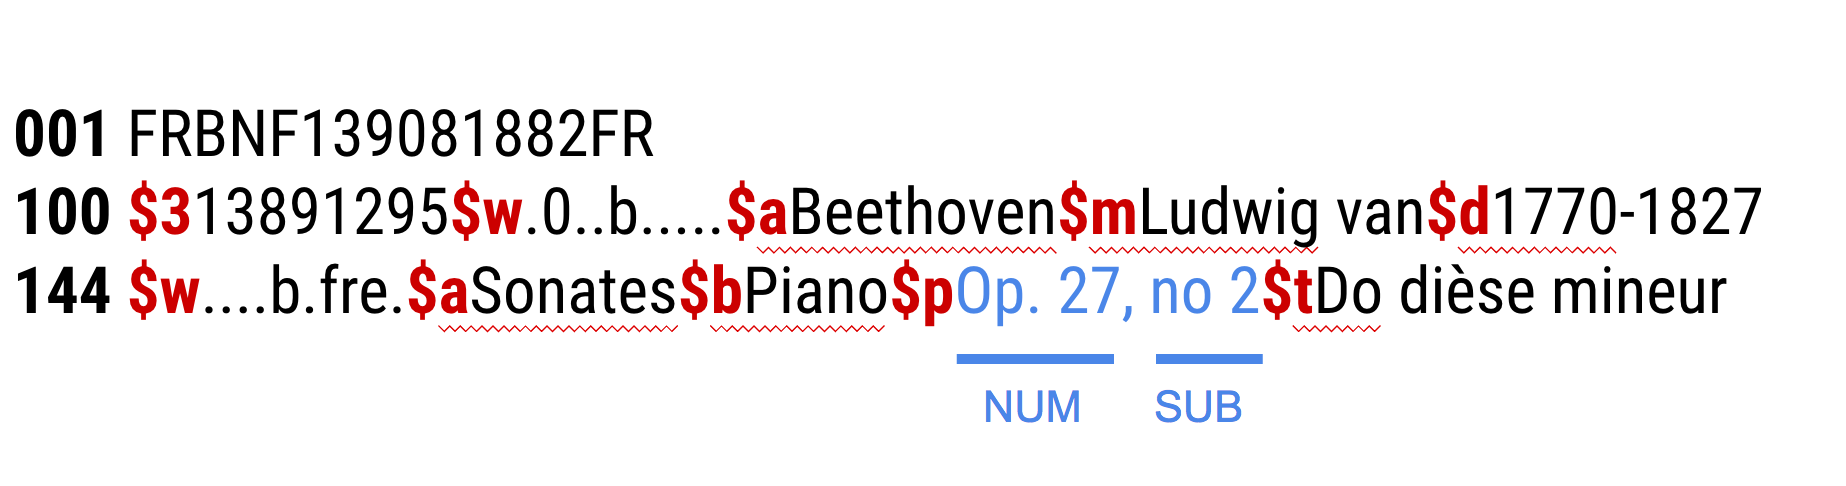
\includegraphics[width=8cm]{MARC_example.png}}}
  \caption{An excerpt of a UNIMARC record.}
 \label{fig:unimarc}
 \smallskip
 \centerline{\framebox{
  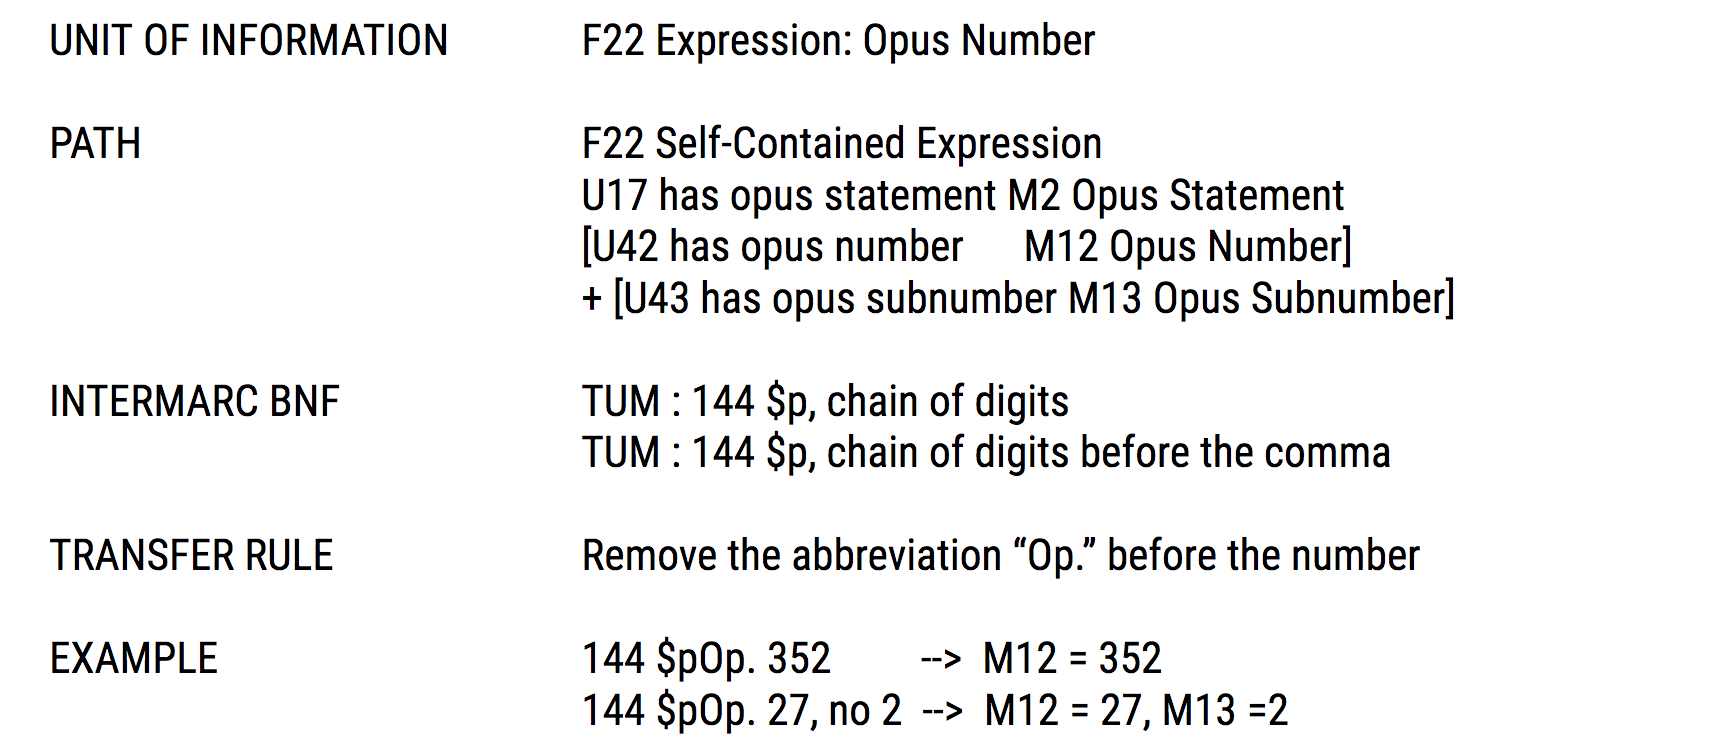
\includegraphics[width=8cm]{mapping_rule.png}}}
  \caption{Example of mapping rules describing the opus number and sub-number of a work}
 \label{fig:mappings}
\end{figure}

\begin{figure}
 \centerline{
 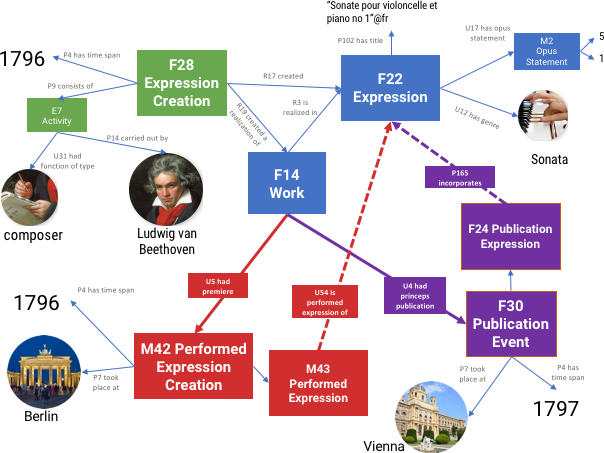
\includegraphics[width=\columnwidth]{schema.png}}
 \caption{Beethoven's \textit{Sonata for piano and cello n.1} represented as a graph}
 \label{fig:schema}
\end{figure}

\section{Musical metadata visualization} \label{visualisation}

We developed the first version of \textsc{Overture} (Ontology-driVen Exploration and Recommendation of mUsical REcords), a prototype of an exploratory search engine for DOREMUS data. \textsc{Overture} is developed as a modern web app, implemented with Node.JS and Angular and available at \url{http://overture.doremus.org}. The application make requests directly to our SPARQL endpoint\footnote{\url{http://data.doremus.org/sparql}} and provide the information to the end-user with a user friendly interface.

The challenge is in giving to the final user a complete vision on the data of each class and letting him/her to understand how they are connected to each other, letting him/her to navigate following the links inside the app. In this way, the user can pass from an artist to his masterpieces, to other works with the same genre.

An advanced search is provided in order to filter the works. The controlled vocabularies plays an important role as possible value of facet filters.

\begin{figure}
 \centerline{
 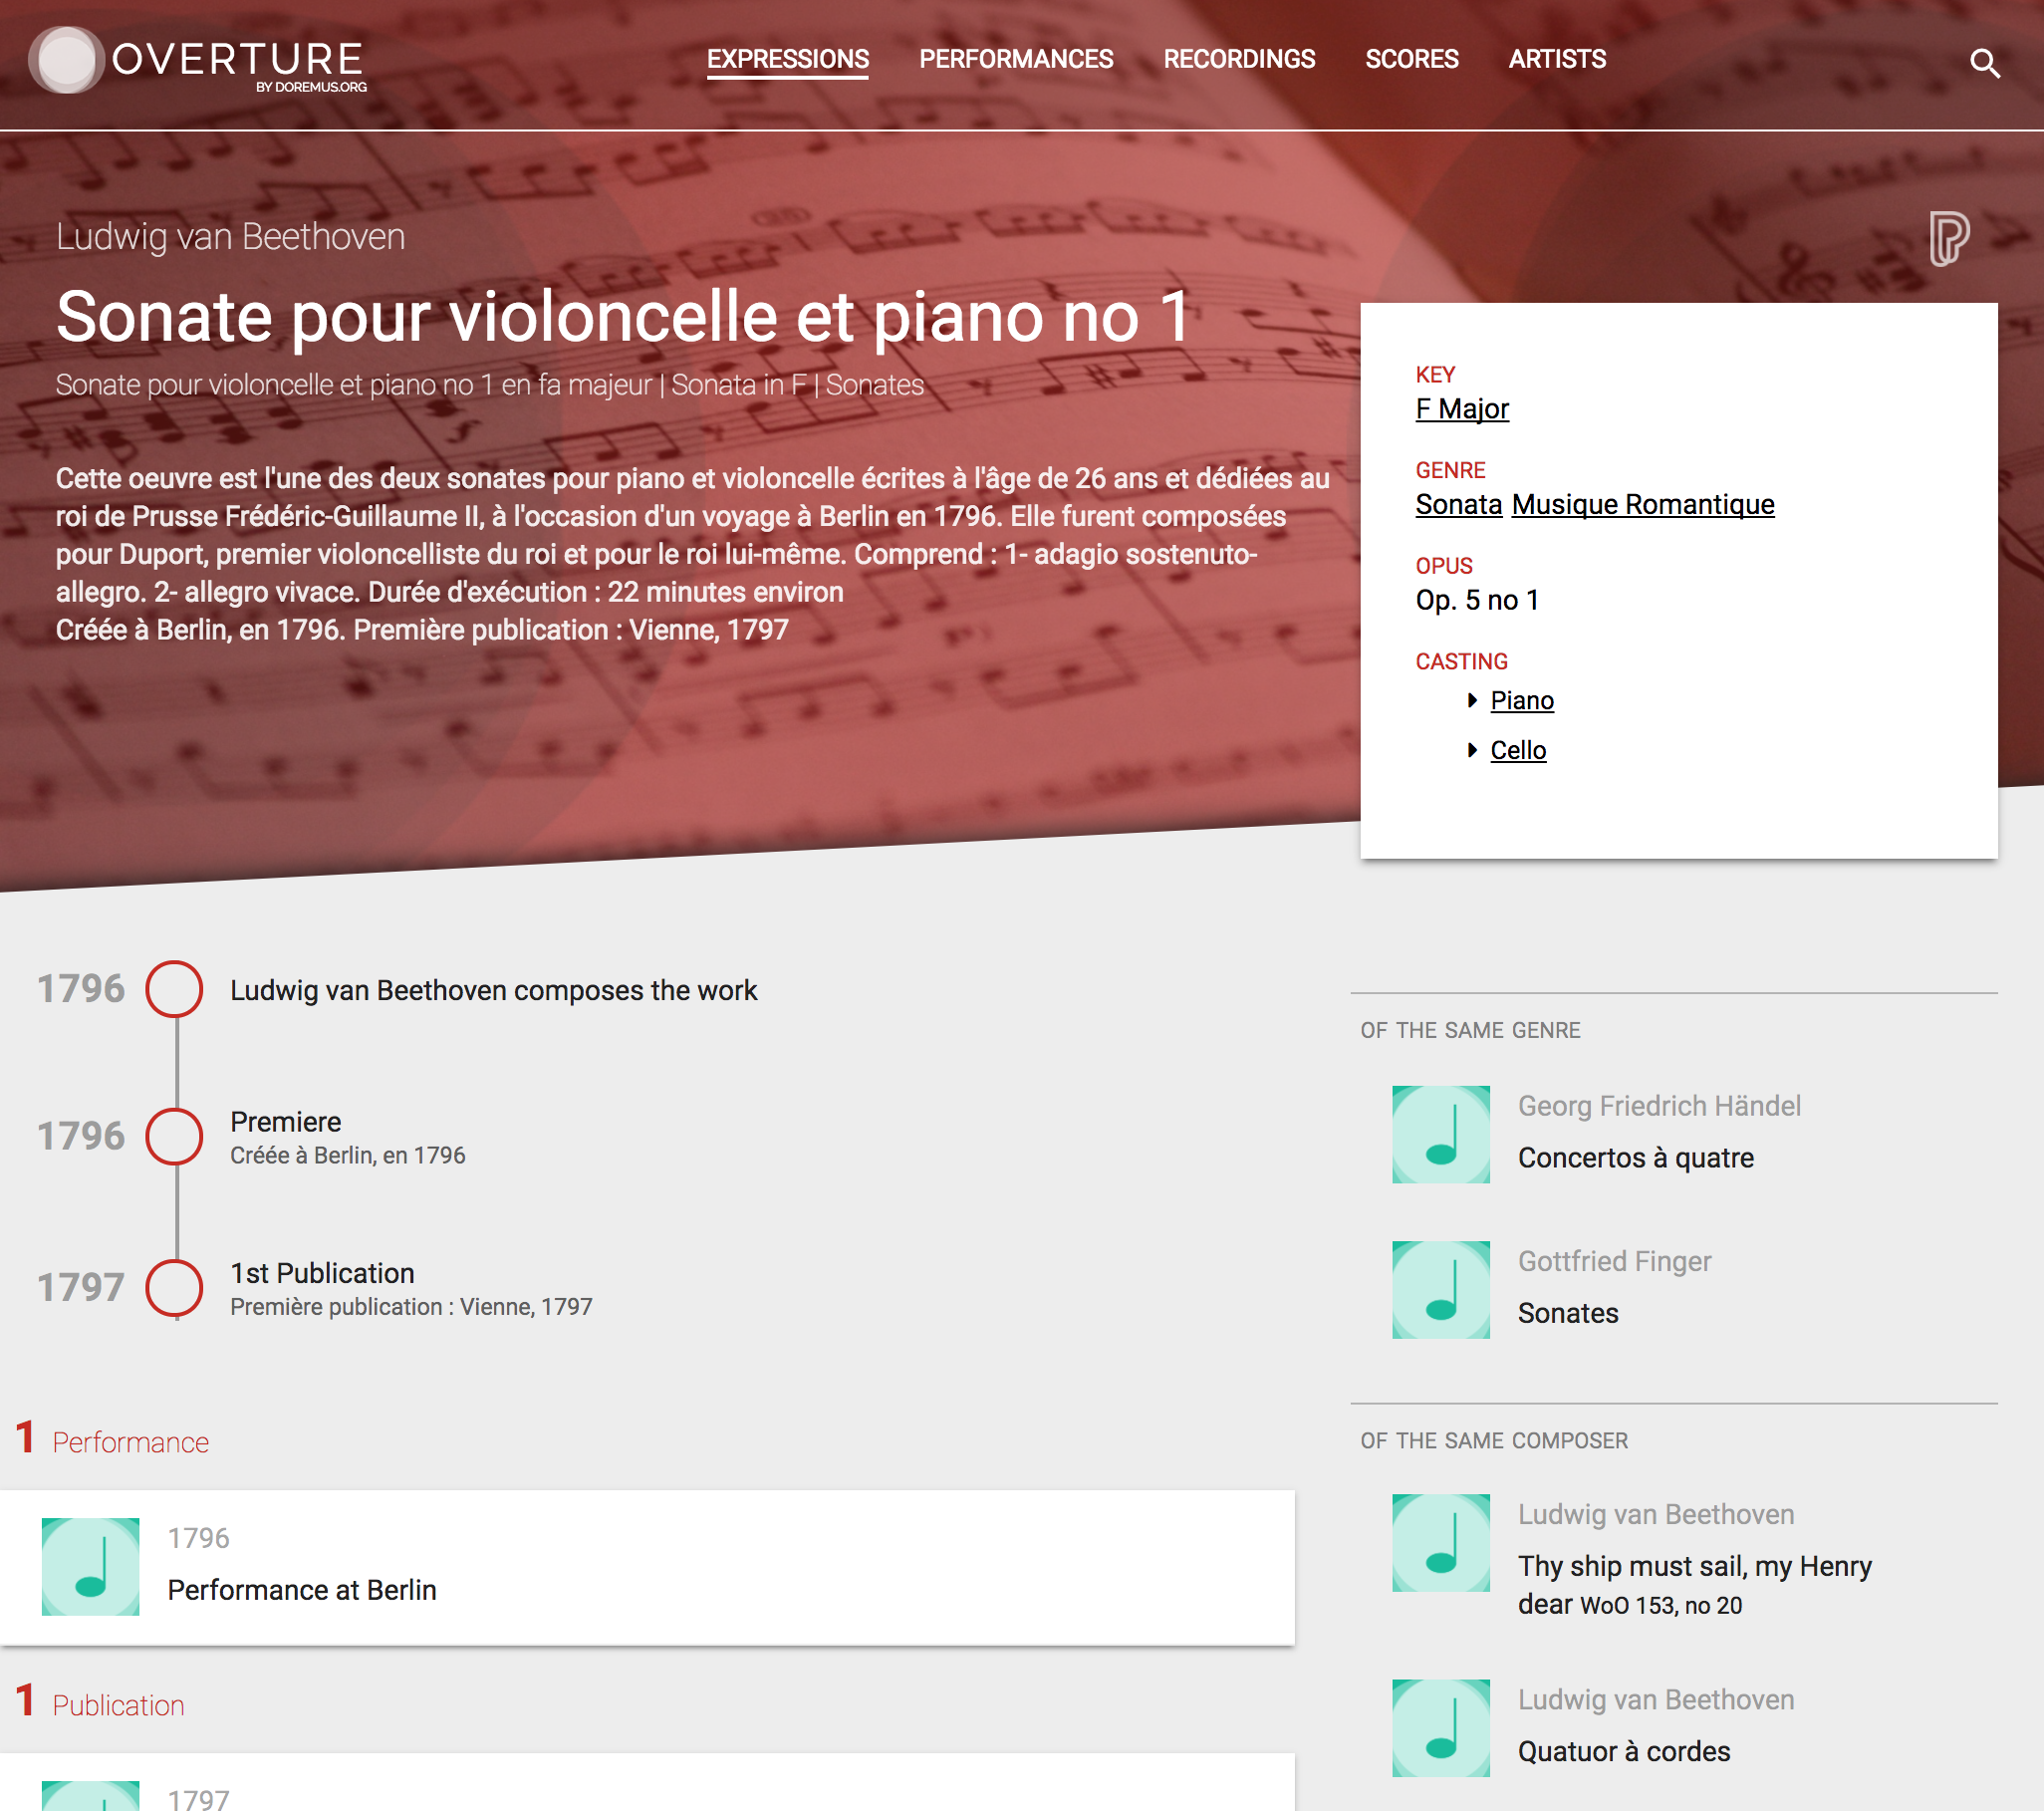
\includegraphics[width=9cm]{overture-sonate-cello.png}}
 \caption{The detail of an expression in \textsc{Overture}}
 \label{fig:overture-detail}
\end{figure}

\section{Recommendation} \label{recommendation}

Our starting point for the study of a suitable algorithm for recommendation consists in two human-made collections. The idea is that this editorial work can be used as a gold standard for training and testing a recommendation system.

We performed an alignment between the tracks of playlists to the data in the DOREMUS knowledge base, using the titles and the names of the artists. We used an extension of the Jaccard similarity measure applied to empirically extracted tokens of the title of each track.

On one side, we have a set of playlists from Radio France web radios. They consists in XML documents with a complex structure, that we convert to a more readable JSON format. Each file covers one day (21 hours) of programs of one radio, and each day is composed of 7 blocks of 3 hours, each one realized by a different editor.
The playlists change once per week, but the difference between two consecutive weeks consists in 1 block only. This means that we have a playlist completely renewed only every 7 weeks. So far, we have access to the entire programming of a single day (so 7 playlists, 1912 tracks, of which 593 were aligned to the DOREMUS knowledge base), but we are waiting for more data soon. 

On the other side, we are studying also the playlist of classical music realized by Spotify and publicly available through a web API. We extracted 80 playlists with a total 4136 tracks, of which 1960 are aligned to the DOREMUS knowledge base.

The main goal of the recommender will be, starting from a seed (a specific work in the DOREMUS dataset), suggest to the user the next work to listen. This task is different from suggesting the most similar one (i.e. the one which the highest number of property in common) because a novelty factor should be included~\cite{celma2009music}.

We are currently studying and running experiments for understanding which recommendation strategy is the best one for our data. We are using \textit{entity2rec}~\cite{palumbo2017entity2rec} (a tool developed by the team) in order to embed the data from the SPARQL endpoint. We are modelling each playlist (or part of it) as a user, and the works in the playlist as the track preferred by the user. Then, the recommendation is performed using a random walk algorithm. Because of the few number of user available to us, the results so far are not satisfactory (the network is not training). We are thinking about dividing long playlist into shorter ones. Another option is using a GAN in order to generate new data. In any case, \textit{entity2rec} should be extended for managing the complexity of our datasets, in which we want to consider also path of properties (e.g. Expression createdBy > consistOf > carriedOutBy Artist) and group of values (e.g. casting mop + casting number + casting responsibility).

In parallel to these collections, we will consider the actual recommendations made by leading music providers. In particular, we are developing ARyTREx\footnote{\url{https://github.com/DOREMUS-ANR/recommender/tree/master/ARyTREx}}, a web application that aims to simulate the recommendations made by Spotify and Last.fm given a seed artist or track and using their respective APIs (\figref{fig:arytrex}). The application enables to collect recommendation paths. We want to use this path as a comparison item for our recommender, asking user feedback for evaluating which recommendation fits better.

\begin{figure}
 \centerline{
 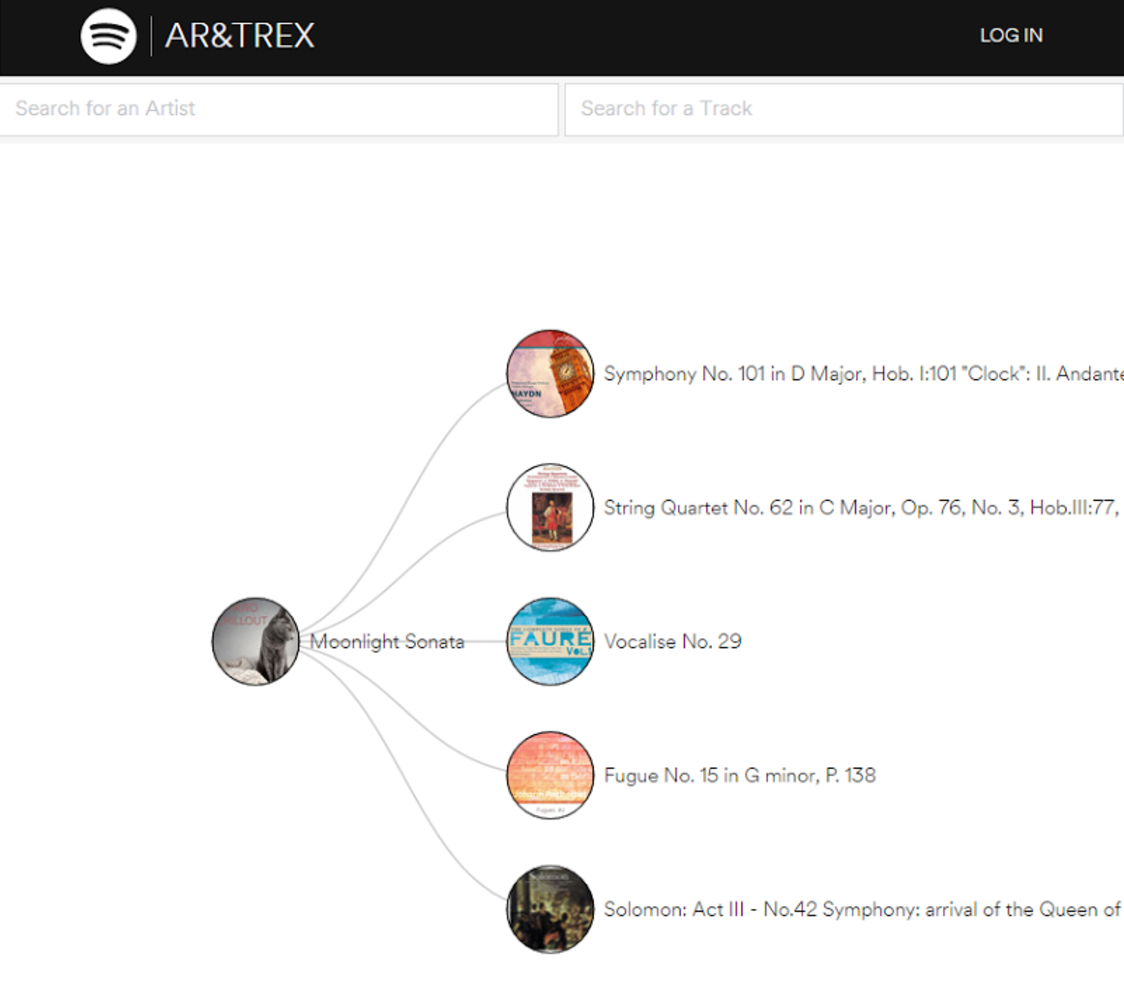
\includegraphics[width=10cm]{arytrex.png}}
 \caption{ArYREx simulate the recommendation of Spotify starting with Moonlight Sonata as a seed.}
 \label{fig:arytrex}
\end{figure}

An experiment of context-based recommendation has been conducted during the supervision of a semester project. The goal of the project was to find connections between Points of Interest (POIs) in a city (we choose Nice as an example) and DOREMUS artists. The system has been implemented by matching to DBpedia both artists (from DOREMUS) and POIs (from 3cixty, a knowledge base for touristic data) and using a tool inspired by RelFinder in order to find the best path between the artist and the POI. The final application is able to suggest to the end-user musical works related to his position and let him discover unexpected and unusual connections (\figref{fig:citymusic}). 

\begin{figure}
 \centerline{
 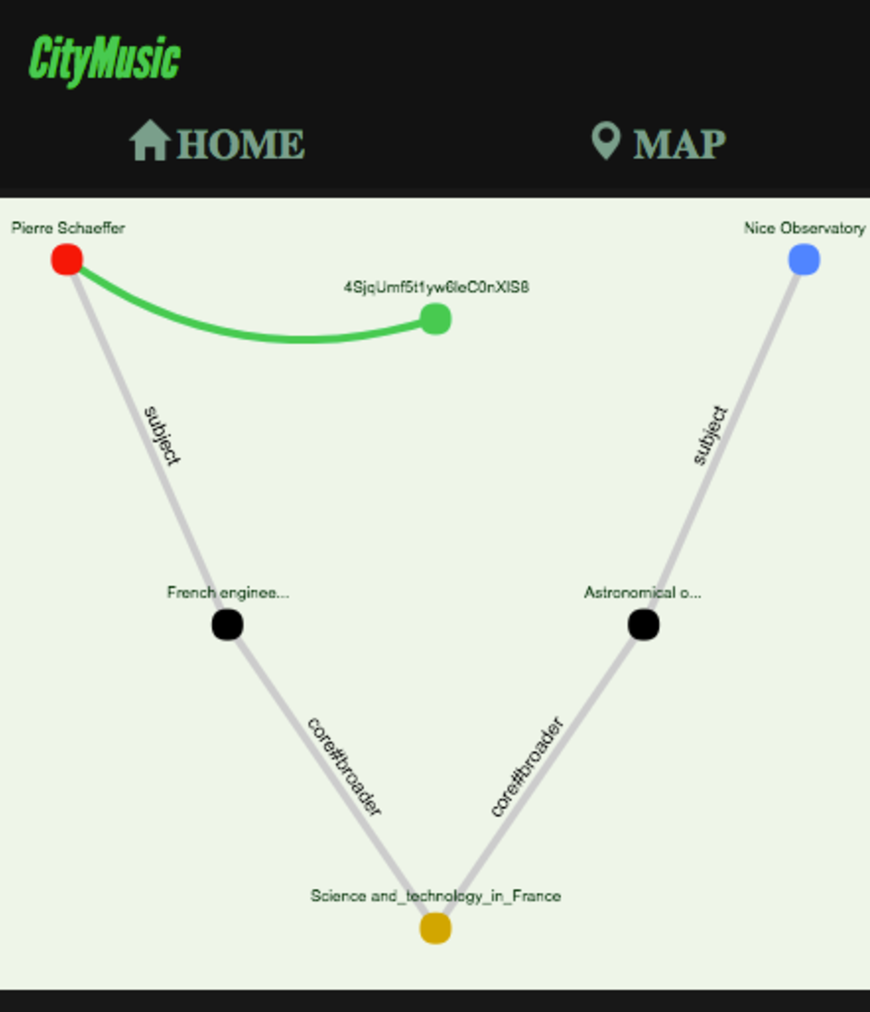
\includegraphics[width=10cm]{citymusic.png}}
 \caption{The artist Pierre Schaeffer was also an engineer. Because of that, CityMusic identified a connection with the Nice Observatory.}
 \label{fig:citymusic}
\end{figure}

%%%%%%%%%%%%%%%
%% Publications
%%%%%%%%%%%%%%%

\chapter*{Publications}
\label{sec:publications}
\ifpdf
    \graphicspath{{Chapter2/Chapter2Figs/PNG/}{Chapter2/Chapter2Figs/PDF/}{Chapter2/Chapter2Figs/}}
\else
    \graphicspath{{Chapter2/Chapter2Figs/EPS/}{Chapter2/Chapter2Figs/}}
\fi

The research carried out during this reporting period has lead to the publication of the following scientific papers:

\section*{Conference}
\begin{enumerate}
\setcounter{enumi}{0}

\item Lisena, Pasquale:
\textbf{Modeling, exploring and recommending music in its complexity.}
EKAW 2016, 20th International Conference on Knowledge Engineering and Knowledge Management, Doctoral Consortium Track, November 19-23, 2016, Bologna, Italy / Also published in Lecture Notes in Computer Science, Vol. 10180

\end{enumerate}


\section*{Poster and Demos}
\begin{enumerate}
\setcounter{enumi}{1}

\item Lisena, Pasquale; Achichi, Manel; Fernandez, Eva; Todorov, Konstantin; Troncy, Rapha\"el
\textbf{Exploring linked classical music catalogs with OVERTURE.}
ISWC 2016, 15th International Semantic Web Conference, Poster Track, October 17-21, 2016, Kobe, Japan.

\item Lisena, Pasquale; Troncy, Rapha\"el:
\textbf{DOREMUS to Schema.org: Mapping a complex vocabulary to a simpler one.}
EKAW 2016, 20th International Conference on Knowledge Engineering and Knowledge Management, Poster Track, November 19-23, 2016, Bologna, Italy / Also published in LNCS, Vol.10180, Springer.

\end{enumerate}

%%%%%%%%%%%%%%
%% Future Work
%%%%%%%%%%%%%%

\chapter*{Future Work}
\label{future}

On the data side, we are working on the improvement of the parsing of the data using Named Entity Recognition (NER) techniques, that will link also the DOREMUS data to external LOD datasets. Regarding the data linking task, although our results on the benchmark data are promising, we still need to address several scaling issues that will allow us to efficiently interconnect our datasets, containing sometimes hundreds of thousands of records. We will be also working on creating links form our data to well-established web knowledge graphs, such as DBpedia.

We are planning to integrate a series of interesting features in \textsc{Overture}, which include the integration of media like images and sound tracks, the retrieving of related information from LOD, and the realisation of a dashboard with interesting and unusual results (along the lines of the Wikipedia homepage). 

Moreover, most of the work will consist in the realisation of the the recommendation system. The recommendation results will be available through API and hosted in the web application.

%\cleardoublepage
\addcontentsline{toc}{chapter}{Bibliography}
\bibliography{doremus}

\end{document}
